\documentclass[options]{article}
\usepackage{tikz}
\usepackage{multirow}
\usepackage{makecell}
\usepackage{array}


\begin{document}
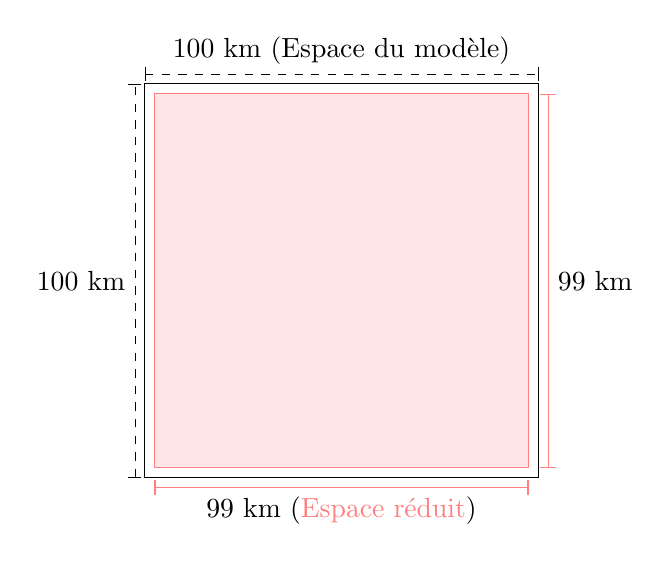
\begin{tikzpicture}[scale=.5]
 \draw[] (0,0) -- (0,10) -- (10,10) -- (10,0) -- cycle;
 \draw[|-|, very thin, dashed] (0, 10.25) -- node[above] {100 km (Espace du modèle)} (10, 10.25);
 \draw[|-|, very thin, dashed] (-0.25, 0) -- node[left] {100 km} (-0.25, 10);
 
 \draw[color=red!50, fill = red!10] (0.25, 0.25) -- (0.25, 9.75) -- (9.75, 9.75) -- (9.75, 0.25) -- cycle;
 \draw[|-|, red!50] (10.25, 9.75) -- node[right,black] {99 km} (10.25, 0.25);
  \draw[|-|, red!50] (0.25, -0.25) -- node[below, black] {99 km ({\color{red!50}Espace réduit})} (9.75, -0.25);
\end{tikzpicture}
\clearpage
\begin{center}
	\begin{tabular}{@{}|>{\centering\arraybackslash}m{.25\textwidth}|>{\centering\arraybackslash}p{.25\textwidth}|>{\centering\arraybackslash}p{.25\textwidth}|>{\centering\arraybackslash}p{.25\textwidth}|@{}}
		\hline
		\textbf{Nom} & \textbf{Variétés} & \textbf{Nombre par défaut en début de simulation} & \textbf{Objectif à atteindre en fin de simulation}  \\
		\hline
		\multirow{3}{*}[-2.5em]{Foyers Paysans} & Nombre & $4 000$ & $4000$ \\
		\cline{2-4}
		 & Part de foyers paysans non mobiles (serfs, esclaves) & $20 \%$ & $20 \%$ \\
		\cline{2-4}
		 & Part de foyers paysans dispersés & $95 \%$ environ & $20 \%$ \\
		 \hline
		\multirow{3}{*}[.5em]{\makecell{Agrégats de\\population}} & Village & $20$ & $200$\\
		\cline{2-4}
		& Agglomération & 4 & 16\\
		\hline
	\end{tabular}  
\end{center}

\end{document}